\tocsection{\textbf{10/28/26 Lecture 26:} Free Groups, Presentations, and Maximal Trees}


\begin{definition}[\textbf{Definition 26.1:} Generators and Free Groups]
    A subset $X$ of a group $G$ is a \emph{set of generators} if each $g \neq e$ can be written as
    \[ g = x_1^{n_1}x_2^{n_2}\cdots x_k^{n_k} \quad \tt{where } x_i \in X,\ n_i \in \Z \setminus \{0\}, \tt{ and } x_i \neq x_{i + 1} \]
    We say $X$ is a \emph{free set of generators} if the representation is unique, and we say $G$ is a \emph{free group}.
\end{definition}

\begin{definition}[\textbf{Definition 26.2:} Words]
    Given an alphabet $X$, a \emph{word} is a finite product $x_1^{n_1}x_2^{n_2}\cdots x_k^{n_k}$ where $x_i \in X$ and $n_i \in \Z$. We say a word is \emph{reduced} if $n_i \neq 0$ and $x_{i + 1} \neq x_i$.
\end{definition}

These form a group in a natural way (concatenation and reduce), called the \emph{free group generated by $X$}, and we denote it $F(X)$.

\begin{example}{\textbf{Example:} Free Group on One Generator}
    It can be easily shown $F(\{x\}) \cong \Z$.
\end{example}

Say $G$ is a group and $X$ is a generating set. This gives us a homomorphism $\phi : F(X) \to G$ by the natural embedding
\[ \phi(x_1^{n_1}\cdots x_k^{n_k}) = x_1^{n_1}\cdots x_k^{n_k} \in G \]
Now, $\phi$ is surjective, so letting $N = \ker(\phi)$, we see
\[ G \cong F(X)/N \]
If $R$ is a collection of words so that $N$ is the smallest normal subgroup containing $R$, we say $\brac{X \mid R}$ is a \emph{presentation} of $G$ with generators $X$ and relations $R$.\\

\textbf{Idea:} We start with the free group $F(X)$ and impose that words in $R$ become the identity.

\begin{definition}[\textbf{Definition 26.3:} Finitely Presented Groups]
    If $X$ and $R$ are finite, we say that the corresponding group $G$ is \emph{finitely presented} and write
    \[ G = \brac{x_1, \ldots, x_n \mid r_1, \ldots, r_{\ell}} \]
\end{definition}

\textbf{Examples:}
\begin{enumerate}
    \item $\brac{x \mid \emptyset} \cong \Z$
    \item $\brac{x \mid x^{n}} \cong \Z/n\Z$
    \item $\brac{x_1, x_2 \mid x_1x_2x_1^{-1}x_2^{-1}} \cong \Z \times \Z$
\end{enumerate}

\begin{definition}[\textbf{Definition 26.4:} Free Products]
    Let $G, H$ be groups. Then, form reduced words $x_1x_2\cdots x_m \in G \cup H$ so that no $x_i$ is the identity of $G$ or $H$, and $x_i$ and $x_{i + 1}$ are not in the same group. Adding the empty word as an identity element, we get a group $G * H$ called the \emph{free product} of $G$ and $H$.
\end{definition}

\textbf{Examples:}
\begin{enumerate}
    \item $\Z * \Z \cong F(\{x_1, x_2\}) =: F_2$.
    \item If $G = \brac{x_1, \ldots, x_m \mid r_1, \ldots, r_k}$ and $H = \brac{y_1, \ldots, y_n \mid s_1, \ldots, s_{\ell}}$, then
    \[ G * H = \brac{x_1, \ldots, x_m, y_1, \ldots, y_n \mid r_1, \ldots, r_k, s_1, \ldots, s_{\ell}} \]
    \item $\Z_2 * \Z_2 = \brac{x \mid x^2} * \brac{y \mid y^2} = \brac{x, y \mid x^2, y^2}$. Now, consider $\phi : \Z_2 * \Z_2 \to \Z_2$,
    \[ \phi(\tt{word}) = \#x\tt{'s} + \#y\tt{'s} \pmod 2 \]
    Then, you can show $\ker(\phi) = \{(xy)^{n}\}_{n \in \Z} \cong \Z$. We call $\Z_2 * \Z_2$ the \emph{infinite dihedral group}.\\

    It turns out $\Z_2 * \Z_2$ can act on $\R$ by $x : u \mapsto -u$ and $y : u \mapsto 2 - u$, which are reflections around $0$ and $1$.
\end{enumerate}

\textbf{Goal:} Our new goal is to compute the fundamental group of simplicial complexes.\\

Let $K$ be a connected simplicial complex. Now, recall that if $f : \abs{K} \to \abs{L}$ is a map and $s$ is a simplicial approximation to $f$, then if $x \in \abs{K}$ and $f(x)$ is a vertex in $\abs{L}$, $f(x) = s(x)$.

\begin{definition}[\textbf{Definition 26.5:} Trees]
    A \emph{tree} in $K$ is a one-dimensional simplicial subcomplex which is simply connected. A tree is \emph{maximal} if no other tree contains it.
\end{definition}

\begin{lemma}[\textbf{Lemma 26.6}]
    A maximal tree in $K$ contains all the vertices.
\end{lemma}
\begin{proof}{Proof:}
    Say $T$ is a maximal tree and suppose a vertex $v$ is not in $T$. Take a vertex $u$ in $T$.\\

    Since $\abs{K}$ is path connected as $\abs{K}$ is connected, there exists a path $\gamma : [0, 1] \to \abs{K}$ from $u$ to $v$. Then, after barycentric subdivision, we can get a simplicial approximation $s : [0, 1] \to \abs{K}$ such that $s(0) = u$ and $s(1) = v$. Now, as $s$ is simplicial, $s$ runs along edges.\\

    Replacing $\gamma$ with $s$, we see $s$ gives us a path $u, v_1, v_2, \ldots, v_k, v$, so as $u$ is in our tree, we can continue building edges along the tree until we get to $v$, either traveling along the tree to get to $v_{i + 1}$, or adding that edge if it doesn't exist. Note that if we ever encounter a vertex on a path not in $T$, adding the edge to $T$ gives us a bigger tree, which contradicts maximality, so we immediately find that $v \in T$. 

    $\qed$
\end{proof}

Now, what we will do is find relations for $\pi_1(\abs{K}, v)$.\\

\textbf{Idea:} Find a maximal tree, and as this is contractible, contract the tree to a point and consider $\abs{K}/T$ (same fundamental group). Each edge not in $T$ becomes a loop in $\abs{K}/T$; these are the generators for $\pi_1(\abs{K}, v)$, and relations come from $2$-simplices in $K$.\\

\textbf{Examples:}
\begin{center}
    \begin{minipage}{0.4\textwidth}
        \centering
        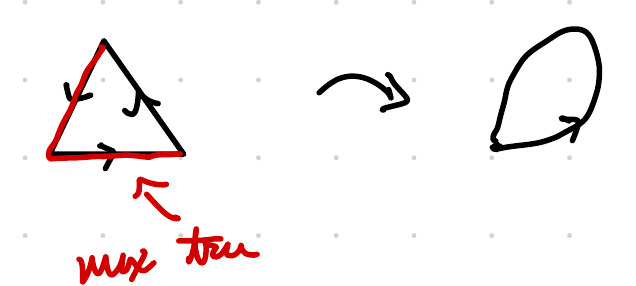
\includegraphics[scale = 0.55]{Lecture26Fig1}
    \end{minipage}
    \begin{minipage}{0.4\textwidth}
        \[ \pi_1(\abs{K}, v) = \brac{\gamma \mid \emptyset} \cong \Z \]
    \end{minipage}\\[0.3cm]
    \begin{minipage}{0.4\textwidth}
        \centering
        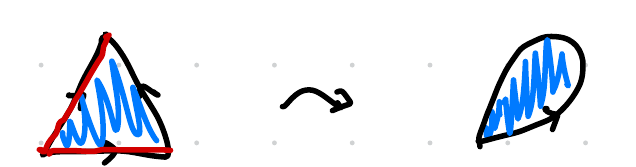
\includegraphics[scale = 0.55]{Lecture26Fig2}
    \end{minipage}
    \begin{minipage}{0.4\textwidth}
        \[ \pi_1(\abs{K}, v) = \brac{\gamma \mid \gamma} \cong \{e\} \]
    \end{minipage}
\end{center}
